\chapter{Optimizing the synthesis of monodisperse colloidal spheres}
\label{ch:synthesis}

\section{Introduction}

The earliest reference to synthetic emulsion polymerization dates back to
1909 \cite{bayer1909,finch03} to a patent awarded to Felix Hoffmann and
co-workers at Farbenfabriken Bayer for the polymerization of diene monomers
in the form of an aqueous emulsion.
\%\% FIXME (maybe) On Wikipedia, the above patent is referenced as the first
suspension polymerization... not emulsion polymerization. 
Techniques for polymerizing emulsions have progressed through
intuitive leaps guided by fundamental principles of chemistry
and physics.  Quite often, the importance of particular chemical
or physical conditions to the outcome can only be gauged once
synthesis is complete, and requires multiple orthogonal measurement
techniques. Examples include measurements of the size distribution
of their particles, their surface texture, and their porosity.
Here, we explore the role of stoichiometry, initiator choice, and
agitation conditions on the synthesis of monodisperse spheres of
\num{3}-methacryloxypropyltrimethoxysilane (TPM) \cite{vanderwel17},
a model system with increasingly widespread applications
in soft-matter research \cite{sacanna11,liu16,vanderwel18}.
We employ holographic particle characterization
in tandem with conventional particle characterization
techniques to identify factors that 
influence size selection, polydispersity, and surface texture.

Spheres made from TPM are a particularly useful system for colloidal studies.
Their synthesis readily produces monodisperse spheres with a size control
between a few hundred nanometers to a few micrometers \cite{liu16} through a process 
that is simpler than that for other common colloidal particles, such 
as polystyrene \cite{goodwin1974} and silica \cite{stober68}. There is no specialized 
equipment or inert environment necessary. However, there are many 
parameters in the synthesis that can affect the average size and refractive
index for a synthesized population. In this chapter we vary a selection of these
conditions and use holographic particle characterization to observe how they affect
emulsion formation and particle polymerization. Our work corroborates and extends
the work of van der Wel \emph{et. al} \cite{vanderwel17} which systematically
characterizes the emulsion polymerization protocol for TPM spheres.

\section{Synthesizing TPM spheres}

Our procedure for synthesizing TPM spheres is nearly identical to the
method established in section \ref{ssec:synthesizing_tpm} with the
exception of initiator choice. We reiterate the synthesis protocol
here to underscore the conditions we varied and to enumerate the
\num{32} samples of droplets and polymerized spheres we analyzed.
A detailed account of the polymer chemistry underlying this
protocol is provided in Ref.~\cite{vanderwel17}.

\subsection{Emulsion polymerization}

The synthesis begins with the formation of an emulsion of TPM droplets.
Monomeric TPM, which is insoluble in water, is added to a basic environment
(pH $>$ \num{9}) of ammonium chloride (\SI{29}{\percent}) in water.
The monomers undergo hydrolysis in water and become water soluble. 
In a basic environment, these hydrolyzed monomers form insoluble 
oligomers. As the suspension is stirred, the oligomers condense 
homogeneously into monodisperse droplets that grow as more oligomers form.
After \num{2} hours, the abundance of free hydrolyzed monomer is depleted
causing oligomerization to halt and therefore droplet growth to cease.
The emulsion is then heated to \SI{80}{\degreeCelsius} and a free radical 
initiator is introduced to polymerize the droplets and form solid spheres.

\% FIXME Where should I put the detailed chemical information?
((3-(Trimethoxysilyl)propyl methacrylate, \SI{98}{\percent}, Sigma Aldrich)

The dissociation of ammonium chloride in water leads to the production of ammonia
gas; as this gas escapes the solution, the pH of the sample decreases.
To lessen this effect, the emulsion formation is completed in a closed vial.
Additionally we use identical \SI{12}{\milli\liter} vials to produce \SI{5}{\milli\liter}
of colloidal suspension in each synthesis so that the amount of enclosed air, and therefore
loss in pH, are approximately equal across samples. As the stirring rod's shape can alter the
flow profile and therefore the droplet properties, we use identical stir bars in all our
studies.

Controlling the size, monodispersity, and composition of colloidal spheres is crucial
for many applications including colloidal crystallization and the self-assembly of
micrometer-sized spheres. In this study we probe the role certain synthesis conditions
have on particle size and refractive index by independently varying specific elements
of the protocol and characterizing the resulting TPM spheres. Specifically,
we investigate the influence of stir rate, concentration of ammonium chloride,
concentration of TPM oil and radical initiator choice on the size and refractive index
of the manufactured particles. To do so, we prepared numerous batches of TPM particles and
characterized the resulting particles with holographic particle characterization

\section{Characterization}

We utilize a Spheryx xSight, a commercial holographic particle characterization system,
to measure the  refractive index and diameter of synthesized TPM spheres.
The xSight flows a colloidal sample through the optical volume of a conventional microscope
that is illuminated by a green laser. The proprietary software and hardware implemented in
the instrument yield the size and refractive index for each observed colloidal spheres and
does so in a fraction of the time we typically spend analyzing an experimental video.
Because we are only interested in collecting population statistics for the size and refractive
index of our colloidal systems, we utilize the xSight rather than our custom-built microscope.

The manufacturer recommends that the particle number density remain below 
\SI{E6}{\milli\liter^{-1}} to reduce the extent to which holograms overlap which
is consistent with our discussion in section \ref{ssec:sample_prep}.
The above emulsification polymerization process produces a sample with a number
density of \SI{E10}{\milli\liter^{-1}} therefore we dilute each of our samples
by a factor of \si{E4}. We utilized \SI{50}{\micro \liter} xCells, the flows cells
designed for the xSight, with each flow analyzing \SI{3}{\micro\liter} of sample;
this provides us with scattering information of a few thousand colloidal spheres per sample.

\begin{figure}
    \centering
    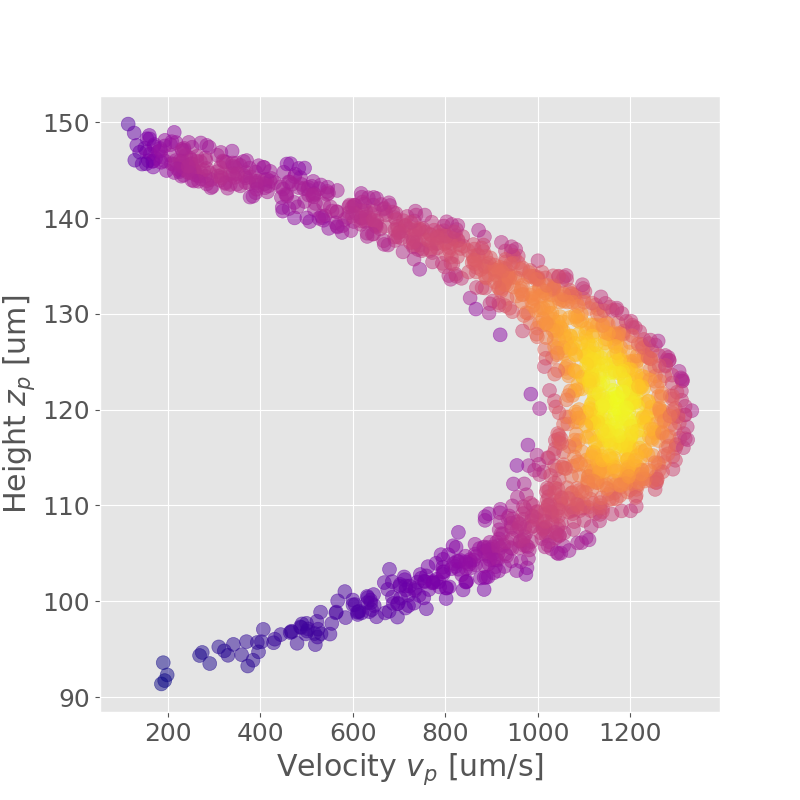
\includegraphics[width=0.5\columnwidth]{example_poiseuille}
    \caption{The recorded Poiseuille flow of particles streaming through the xCell. The
      color denotes the density of observations. \%FIXME: add color bar.}
    \label{fig:flow_prof}
\end{figure}

The flow cell is at rest while the dilute suspension flows above
the field of view producing a Poiseuille flow of fluid through the
xCell. Because the xSight records the mean $z$-position and mean 
velocity of all multiply-imaged scatterers, we are able to fit the flow
profile to a Poiseuille flow as depicted in Fig.~\ref{fig:flow_prof}.
To refine the population estimates of refractive index and diameter, 
we filter the data which deviates from our parabolic fit by more 
than one median absolute deviation.

\section{Results}
\subsection{Effect of stir rate}

Stirring the sample as the oligomers condense into droplets suppresses coalescence and
promotes homogeneous nucleation by uniformly dispersing the hydrolyzed monomer and droplet
nuclei. %%FIXME CHECK THIS STATEMENT.
The effect stir rate has on the resulting particle size is, however, less clear;
we investigated the influence of stir rate by producing \num{4} sets of TPM emulsions.
In four identical vials with identical stir bars, we placed \SI{15}{\milli\liter} of 
\SI{29}{\percent} ammonia followed by \SI{200}{\micro\liter} of TPM 
monomer to \SI{5}{\milli\liter} of DI water. The four samples were then stirred 
using magnetic stir plates set at \num{500}, \num{700}, \num{900}, and
\SI{1100}{\minute^{-1}} for \SI{2}{\hour}. % XXX Use rpm instead of min^{-1}?
The droplets were then polymerized by adding
\num{2},\num{2}'-azobis(\num{2}-methylpropionitrile) (AIBN) as a radical initiator and 
heating the sample to \SI{80}{\celsius} for \SI{2}{\hour}.
We prepared samples of the unpolymerized droplets and polymerized TPM spheres such that
there were \num{8} sets of data (\num{2} sets for each spin rate) suitable for holographic
characterization.

Scanning electron microscopy (SEM) images of the polymerized particles were taken with a
MERLIN (Carl Zeiss) field emission scanning electron microscope and are provided in
Fig.~\ref{fig:synthesis_stir_rate}(a). SEM images provide a visual check on the monodispersity
and an approximate size of individual colloidal spheres. While a well calibrated scanning
electron microscope provides \num{1} to \SI{10}{\nm} resolution of features, sample
preparation, particularly vacuum decompression and sputter coating, can shrink or
even swell the sample \cite{yamada85,jung02}. We utilized ImageJ to analyze \num{10}
particle in each frame. The average particle diameters were \SI{1.48}{\um}, \SI{1.63}{\um},
\SI{2.03}{\um}, and \SI{1.82}{\um} for stirring rates \num{500}, \num{700}, \num{900}, and
\SI{1100}{\minute^{-1}} respectively. We note that the SEM images for the emulsion
stirred at \SI{1100}{\minute^{-1}} reveal a small population of \SI{100}{\nm}.

The result of holographic particle characterization for the \num{4} polymerized samples
and the \num{4} unpolymerized samples are summarized in Fig.~\ref{fig:synthesis_stir_rate}(b).
Each dot represents the average size and refractive index for the associated sample. Error
bar length is set by a single median absolute deviation of the associated property.
The unpolymerized droplets, represented with dashed error, bars have a categorically
lower refractive index than the polymerized droplets, represented with solid error bars.
Polymerization changes the chemical makeup of the droplet and generally increases the
density between the two states; both processes can increase the refractive index
of the particle and can certain account for the modest $\sim\SI{2}{\percent}$ %FIXME Citation.
The refractive index shift from the monomeric TPM oil to the unpolymerized droplets
is substantial.
condensed oligomerized TPM


\begin{figure}
    \centering
    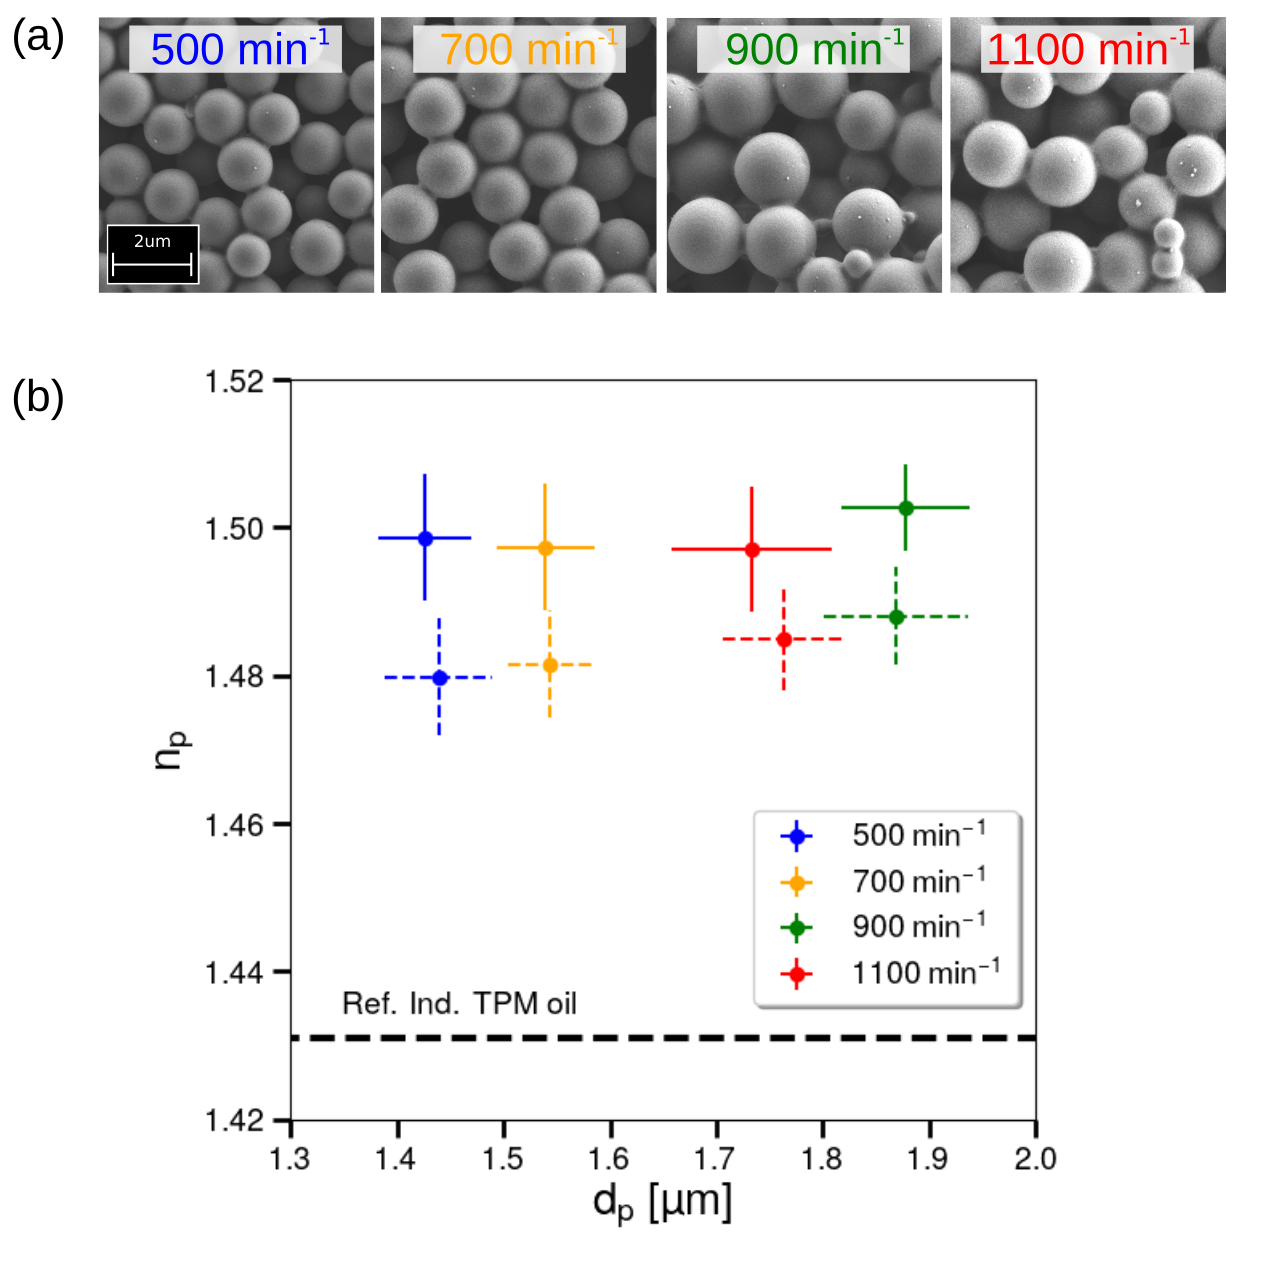
\includegraphics[width=\columnwidth]{synthesis_stir_fig}
    \caption{(a) Cropped and scaled FESEM images of the polymerized TPM spheres whose
      samples were stirred at \num{500}, \num{700}, \num{900}, and \SI{1100}{\minute^{-1}}.
      (b)  The result of HPC analysis for the unpolymerized and polymerized
      emulsions stirred at \num{4} different rates. Solid-lines represent the polymerized
      spheres; dashed-lines represent the unpolymerized droplets; color differentiates the sample by
      spin rate. Each dot represents the
      average diameter and refractive index for a sample. Error bars are set by a single
      median absolute deviation of the measured property for a given sample. The dashed
      black line provides reference to the refractive index of monomeric TPM oil.}
    \label{fig:synthesis_stir_rate}
\end{figure}

Next we investigate the time evolution of
polymerized droplets as a function of their exposure to the heat bath. Specifically, we draw
samples from a 
We synthesized a total of \num{32} batches of TPM particles including droplets and solid
spheres. The stir rate, amount of ammonia added, the amount of monomeric TPM oil added
and the heat bath exposure time were all probed.

\subsection{Emulsion formation}

To probe the variables of droplet formation, we make four batches of droplets.
In each case we hold the volume of water, \SI{5}{\milli \liter} constant 
and vary the amounts of TPM and ammonia. Batches A and B each had 
\SI{100}{\micro\liter} of TPM with \si{10} and \SI{20}{\micro\liter} of 
ammonia added, respectively. Batches C and D had \SI{150}{\micro\liter}, 
again with \si{10} and \SI{20}{\micro\liter} of ammonia, respectively. 
\SI{0.1}{\percent} sodium docecyl sulfate (SDS) was introduced to
each sample to suppress aggregation. Through this, we can observe the effects of
varying the amount of TPM and the pH on the size of the resulting droplets.
This gives 
% XXX (Add conclusions about initiator- does not seem to matter)

\subsection{Polymerization}

The polymerization of the TPM droplets can be tracked by observing the 
refractive index of the particles over time. As the droplets polymerize, 
their refractive index increases until they are fully polymerized. To track 
this, we sampled the suspension above that was stirred at \SI{1100}{\min^{-1}}
% XXX Again, rpm vs mins^{-1}
after \si{5}, \si{10}, \si{15}, \si{20}, \si{40}, and \SI{60}{\min} of 
heating and measured the particles' refractive index. 
%XXX (Add conclusions about polymerization time- only takes maybe 15 min?)

Next, we observe the effect of using different free radical initiators 
to polymerize the particles. Two water-insoluble initiators, AIBN and
\num{1},\num{1}'-azobis(cyclohexanecarbonitrile) (ACHN), and two water-soluble 
initiators, potassium persulfate (KPS) and ammonium persulfate APS), were 
used.

To compare initiators, one \SI{5}{\milli \liter} suspension of emulsion droplets is
made in a \SI{12}{\milli \liter} vial and then equally divided into five
\SI{1.5}{\milli \liter} microcentrifuge tubes. One tube was left unpolymerized. The
other four tubes were then polymerized at \SI{80}{\celsius} 
for \SI{12}{\hour} on a shaker at \SI{750}{\minute^{-1}} % XXX Again, rpm vs mins^{-1}
to prevent sedimentation.
We added a different free radical initiator to each tube and repeated the process with four
different emulsions for a total of 
\num{16} measurements to ensure that any observations were the result of the 
initiator used and not of the particular protocol used to make the emulsion.

\section{Results}


% Van Der Wel et. al suggest that the density increases by 1.07 during polymerization.
% IF the mass stays the same, this corresponds to a 2% decrease in radius.
% For a 1.5 um diameter TPM sphere, a 2% decrease reduces the size to 1.46 um.
% That would be visible in our 

\subsection{Role of emulsion conditions}
\%(This title is terrible)


\begin{figure}
    \centering
    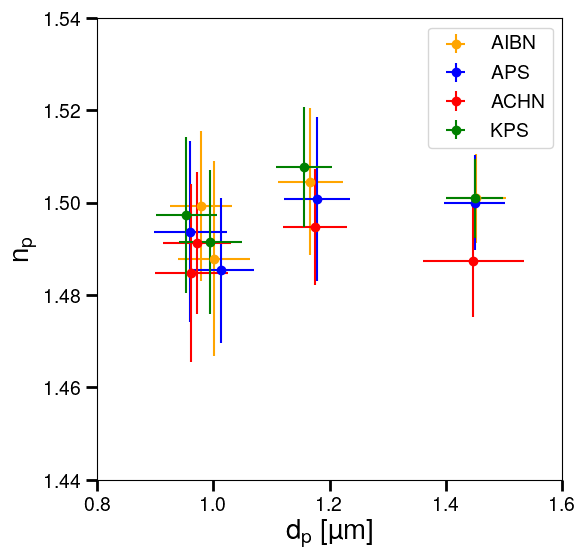
\includegraphics[width=0.75\columnwidth]{may_data_summary.png}
    \caption{The refractive index and diameter of 16 samples of 
    polymerized TPM.}
    \label{fig:initiator_data}
\end{figure}

In making the \si{16} sets of particles to look at the effect of initiator on 
the particles, we can also make observations about the effects of varying 
the amount of TPM and the pH on the size of the resulting droplets. To hold 
the pH constant, we can compare sample A to C and sample B to D. This gives 
the fairly intuitive result that increasing the amount of TPM increases the 
size of the final droplet. Holding the amount of TPM constant and varying 
the pH, which means comparing A to B and C to D, shows that increasing the 
pH of the environment during droplet formation decreases the size of the 
final droplet. This is less intuitive but perhaps not surprising, as the pH 
affects the rate at which oligomers form and therefore the rate of droplet 
formation. This leads to more nucleation sites and therefore smaller droplets 
for the same volume of material. 

Comparing batches A to C, each with \SI{100}{\micro \liter} of TPM monomer, and B to D with
\SI{150}{\micro \liter}, gives the somewhat intuitive result that increasing the amount of TPM
monomer increases the size of the final droplet. On the other hand, comparing A to B with
\SI{10}{\micro \liter} ammonia and C to D with \SI{15}{\micro \liter} ammonia shows that
increasing the pH of the environment during droplet formation decreases the size of the 
final droplet. This is less intuitive but perhaps not surprising, as the pH 
affects the rate at which oligomers form and, therefore, the rate of droplet 
formation. Increasing the pH results in more nucleation sites and therefore smaller droplets 
for the same volume of material. 

\subsection{Role of Initiator.}

Under certain conditions, TPM droplets are known to form dimpled spheres when polymerized with
the water-soluble initiators APS and KPS due to the ejection of low molecular weight oligomers
(citation- I forget which of Stefano's papers?). Therefore, one might think that TPM spheres
polymerized with these initiators would be made of on average higher molecular weight oligomers
and have a higher refractive index than pa. However, under the conditions observed here where no
dimple was formed, there was no observable difference in particle size or refractive index between
the initiators used.

\subsection{Role of Heat Bath.}


\begin{figure}
    \centering
    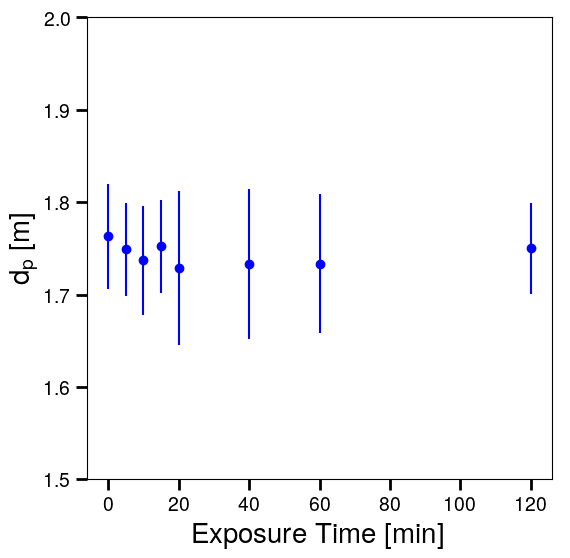
\includegraphics[width=0.9\columnwidth]{may_data_heat_bath_size_time}
    \caption{Caption}
    \label{fig:heat_size_time}
\end{figure}



\begin{figure}
    \centering
    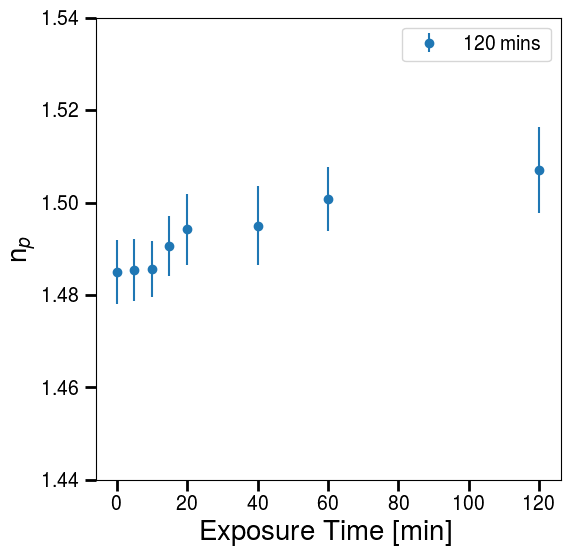
\includegraphics[width=0.9\columnwidth]{may_data_heat_bath_time}
    \caption{Caption}
    \label{fig:heat_ref_time}
\end{figure}

\section{Discussion}

\section{Acknowledgment}

This work was supported primarily by the MRSEC program of
the National Science Foundation through Award Number DMR-1420073.
Additional support was provided by the SBIR program of the
National Science Foundation through Award Number IPP-1519057.
The FESEM was purchased with financial support from the MRI program
of the National Science Foundation under Award DMR-0923251.

\% FIXME David please check the acknowledgment
